\chapter{Hasil dan Analisis}

Kecuali disebutkan lain, angka pada bab ini adalah Macro F1 dari prediksi out-of-fold (OOF) 5-fold pada 27.309 baris data latih hasil dedupe, dengan threshold yang dipilih dari OOF. Data uji tidak dipakai untuk memilih konfigurasi. Skor public adalah skor leaderboard Kaggle dari berkas submission yang diunggah.

\section{Ringkasan Model Terbaik}

\begin{table}[H]
\centering
\caption{Model terbaik tiap algoritma from scratch}
\label{tab:ringkasan}
\begin{tabularx}{\textwidth}{>{\raggedright\arraybackslash}p{2.6cm}X rr}
\toprule
Model & Konfigurasi & OOF & Public \\
\midrule
\textbf{KNN + kembar} & Minkowski $p=1{,}5$, $k=17$, bobot $1/d^2$, preprocessing bersama, vote booking kembar & \textbf{0,8529} & \todo{skor} \\
KNN & Sama, tanpa vote booking kembar & 0,8476 & -- \\
DTL & Gain ratio (C4.5), depth 30, leaf 5, min gain $2\times10^{-4}$ & 0,8343 & 0,84679 \\
LR & L2, bin berbasis target, interaksi, sel dua dimensi (\texttt{lr\_cross\_bins}) & 0,8344 & 0,83542 \\
SVM & Gaussian, $C=0{,}3$, $\gamma=1$, preprocessing template & 0,8324 & 0,85189 \\
NB & Categorical kontekstual, sembilan masukan, $\alpha=0{,}1$ & 0,8020 & 0,80173 \\
\bottomrule
\end{tabularx}

\end{table}

KNN dengan vote booking kembar adalah model final kelompok dan mencapai \textbf{peringkat 1} pada public leaderboard. \todo{tulis skor public dan private akhir}. Notebook \texttt{src/main.ipynb} mereproduksi berkas submission tersebut secara identik, dengan md5
\begin{center}\texttt{39505c42f93d193ce99a023cabd3e9d9}\end{center}

\section{Hasil K-Nearest Neighbors}

\subsection{Baseline}
Baseline memakai $k=5$, jarak Euclidean, voting seragam, dan 39 kolom hasil imputasi, one-hot, dan standardisasi z-score tanpa fitur turunan (notebook \texttt{knn\_baseline}).

\begin{table}[H]
\centering
\caption{KNN baseline: from scratch vs scikit-learn}
\label{tab:knn_baseline}
\begin{tabular}{lrr}
\toprule
Metrik & From scratch & scikit-learn \\
\midrule
Macro F1 OOF (threshold 0,41) & 0,7632 & 0,7632 \\
Std antar-fold & 0,0034 & 0,0034 \\
F1 kelas 0 / kelas 1 & 0,8519 / 0,6746 & identik \\
Selisih probabilitas OOF maksimum & \multicolumn{2}{c}{0 (identik pada 27.309 baris)} \\
Waktu CV 5-fold & sekitar 92 detik & sekitar 9 detik \\
\bottomrule
\end{tabular}
\end{table}

\begin{figure}[H]
\centering
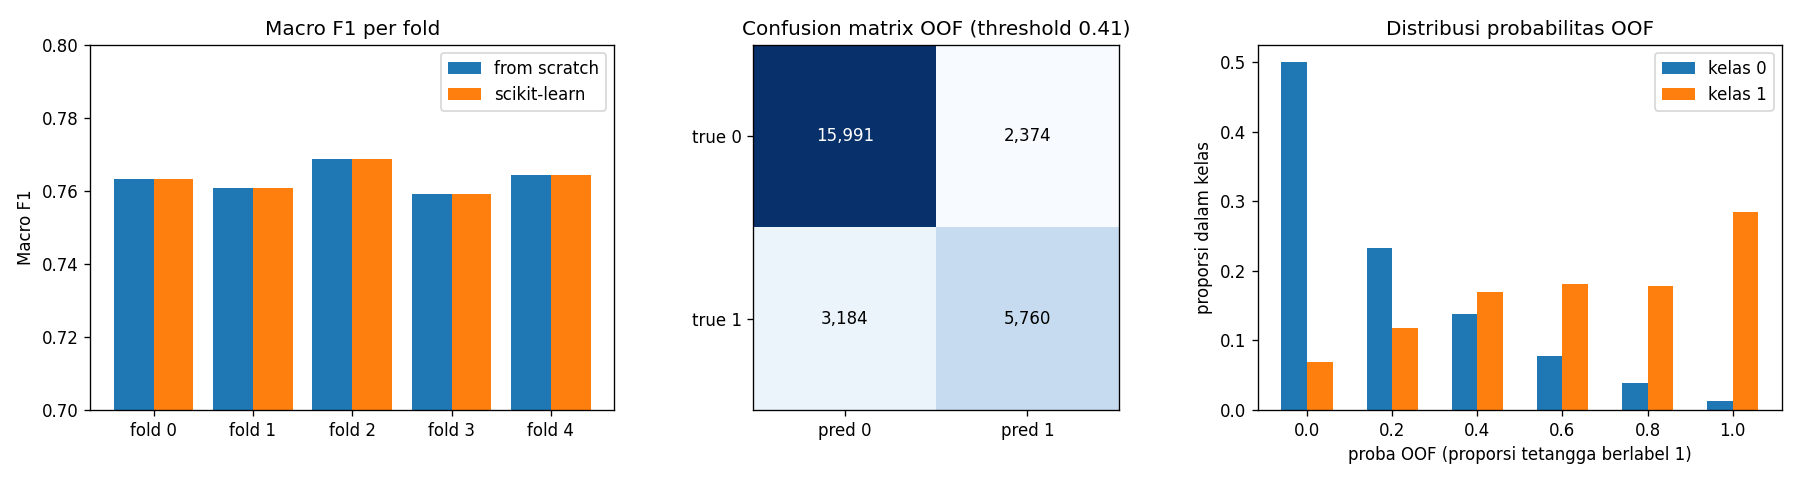
\includegraphics[width=\textwidth]{knn_baseline_comparison.png}
\caption{KNN baseline: Macro F1 per fold, confusion matrix OOF, dan distribusi probabilitas OOF}
\label{fig:knn_baseline}
\end{figure}

\begin{figure}[H]
\centering
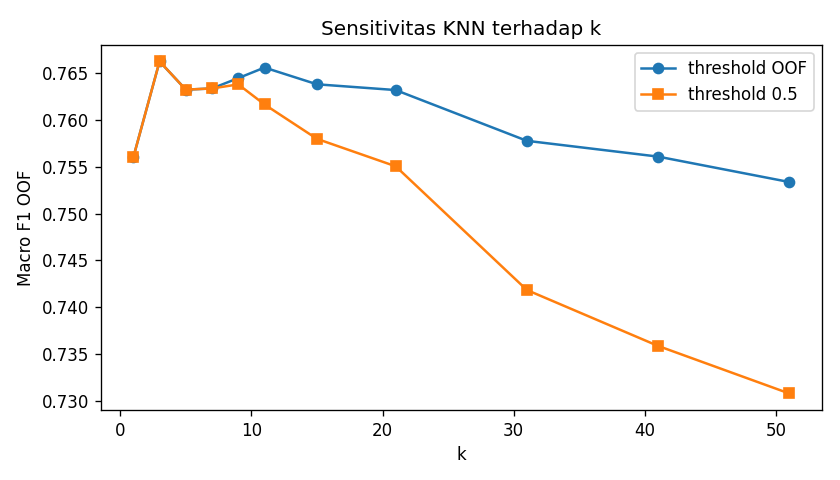
\includegraphics[width=0.65\textwidth]{knn_baseline_k_sweep.png}
\caption{Sensitivitas $k$ pada KNN baseline}
\label{fig:knn_ksweep}
\end{figure}

\subsection{Perkembangan KNN}

\begin{table}[H]
\centering
\caption{Perkembangan konfigurasi KNN sampai model final}
\label{tab:knn_progres}
\begin{tabularx}{\textwidth}{>{\raggedright\arraybackslash}p{4.6cm}X rr}
\toprule
Notebook & Perubahan & OOF & Public \\
\midrule
\texttt{knn\_baseline} & Euclidean, $k=5$, seragam, 39 kolom & 0,7632 & -- \\
\texttt{knn\_forward\_selection} & Forward selection 7 fitur, Manhattan, $k=15$, vote terbobot jarak & 0,8373 & 0,84872 \\
\texttt{knn\_selection\_distance} & Seleksi fitur dengan vote terbobot jarak, 8 fitur, $k=19$ & 0,8411 & 0,85505 \\
\texttt{knn\_feature\_weight} & Bobot fitur hasil coordinate search & 0,8453 & 0,85469 \\
\texttt{knn\_robust\_clip\_minkowski\_weighted} & Dedupe, data error, clipping, robust scaler, $p=1{,}5$, bobot $1/d^2$, $k=19$, 15 fitur & 0,8481 & 0,864 \\
\texttt{knn\_robust\_clip\_minkowski\_weighted\_twin} & + vote booking kembar (toleransi lead 5 hari, tanggal 5 hari) & 0,8520\textsuperscript{b} & 0,87119 \\
model final (\texttt{src/main.ipynb}) & Toleransi lead 10 hari, tanggal 2 hari, harga 6\%, $\alpha=0{,}8$, threshold 0,4845 & 0,8531\textsuperscript{b} & \todo{} \\
\bottomrule
\end{tabularx}

\raggedright\footnotesize \textsuperscript{b} Rata-rata OOF pada tiga seed fold (4, 5, 42) dengan threshold tetap, karena perbedaan antarkonfigurasi kembar sangat kecil.
\end{table}

\subsection{Model final: KNN dengan vote booking kembar}

\begin{table}[H]
\centering
\caption{KNN final: holdout, OOF, dan perbandingan dengan scikit-learn}
\label{tab:knn_final}
\begin{tabular}{lr}
\toprule
Metrik & Nilai \\
\midrule
Macro F1 holdout, KNN + kembar & 0,8592 \\
Macro F1 holdout, KNN saja & 0,8539 \\
Macro F1 OOF 5-fold, KNN + kembar (threshold 0,4845) & 0,8529 \\
Macro F1 OOF 5-fold, KNN saja & 0,8476 \\
Confusion matrix OOF [TN, FP; FN, TP] & [16.728, 1.637; 1.877, 7.067] \\
F1 kelas 0 / kelas 1 (OOF) & 0,9049 / 0,8009 \\
Macro F1 holdout KNN scikit-learn vs from scratch & 0,8539 vs 0,8539 \\
Selisih probabilitas maksimum terhadap scikit-learn & sekitar $10^{-7}$ \\
\bottomrule
\end{tabular}
\end{table}

\begin{figure}[H]
\centering
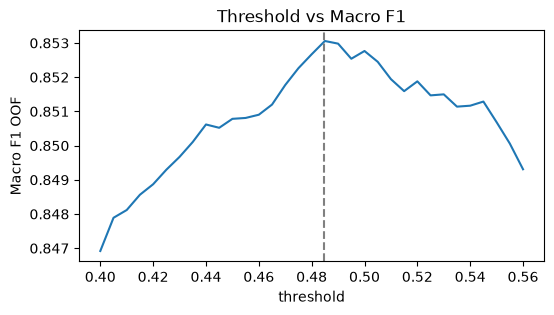
\includegraphics[width=0.6\textwidth]{knn_threshold.png}
\caption{Macro F1 OOF KNN final terhadap threshold}
\label{fig:knn_threshold}
\end{figure}

Setiap pilihan preprocessing dan parameter kembar diuji ulang dengan mengganti satu pilihan dan mempertahankan yang lain (Tabel~\ref{tab:knn_audit}). Semua angka adalah rata-rata OOF pada tiga seed fold dengan threshold 0,48.

\begin{table}[H]
\centering
\caption{Uji pilihan preprocessing dan vote kembar (rata-rata OOF 3 seed fold)}
\label{tab:knn_audit}
\small
\begin{tabular}{llr}
\toprule
Bagian & Varian & OOF \\
\midrule
Dasar & robust, clip 0,5\%, median, $1/d^2$, kembar 10/2/5\% & 0,8528 \\
\midrule
\multirow{3}{*}{Scaler} & z-score & 0,8498 \\
 & rank & 0,8463 \\
 & min-max & 0,8444 \\
\midrule
\multirow{3}{*}{Missing} & imputasi sebelum fitur turunan & 0,8524 \\
 & kategori kosong menjadi one-hot nol & 0,8513 \\
 & jarak mengabaikan kolom kosong & 0,8465 \\
\midrule
\multirow{2}{*}{Bobot vote} & $1/d$ & 0,8516 \\
 & Gaussian & 0,8473 \\
\midrule
\multirow{3}{*}{Clipping} & persentil 1\% & 0,8525 \\
 & IQR $\times3$ & 0,8529 \\
 & tanpa clipping & 0,8529 \\
\midrule
\multirow{3}{*}{Toleransi kembar} & lead 5, tanggal 5 hari & 0,8520 \\
 & lead 12, tanggal 2 hari & 0,8526 \\
 & harga 0\% / 2\% / 10\% & 0,8497 / 0,8521 / 0,8523 \\
\midrule
\multirow{4}{*}{Bobot kembar} & $\alpha$ = 0,5 / 0,6 & 0,8516 / 0,8525 \\
 & $\alpha$ = 0,9 / 1,0 & 0,8524 / 0,8506 \\
 & minimal 1 kembar & 0,8511 \\
 & minimal 3 kembar & 0,8527 \\
\midrule
Final & harga 6\%, $\alpha=0{,}8$, threshold 0,4845 & \textbf{0,8531} \\
\bottomrule
\end{tabular}
\end{table}

\subsection{Analisis KNN}
\begin{enumerate}
  \item \textbf{Kebenaran implementasi.} Pada baseline, probabilitas OOF from scratch identik dengan scikit-learn di seluruh 27.309 baris. Pada konfigurasi final, selisih probabilitas maksimum hanya sekitar $10^{-7}$ (presisi float32) dan Macro F1 holdout sama persis.
  \item \textbf{Representasi fitur paling menentukan.} KNN yang sama naik dari 0,7632 ke 0,8481 hanya dengan seleksi fitur, bobot fitur, robust scaler, clipping, dan jarak Minkowski $p=1{,}5$. Fitur yang tidak relevan ikut menentukan jarak dengan bobot yang sama, sehingga membuangnya memberi kenaikan terbesar.
  \item \textbf{Robust scaler dan jarak $p=1{,}5$.} Z-score, min-max, dan rank terpengaruh ekor panjang lead time dan harga. Jarak $p=1{,}5$ berada di antara Manhattan dan Euclidean sehingga satu kolom dengan selisih besar tidak terlalu mendominasi.
  \item \textbf{Vote booking kembar.} Pemesanan kembar hampir selalu berlabel sama (93,2\%), tetapi lead time-nya berbeda beberapa hari karena noise. KNN biasa dapat melewatkan kembar ini, sedangkan vote kembar memakainya secara langsung. Holdout naik dari 0,8539 ke 0,8592 dan OOF dari 0,8476 ke 0,8529. Toleransi lead time 10 hari lebih baik daripada 5 hari, sesuai temuan bahwa noise ada pada lead time.
  \item \textbf{Area yang datar.} Variasi parameter kembar di sekitar konfigurasi final hanya mengubah OOF sekitar $\pm0{,}001$. Konfigurasi berada di area yang stabil, bukan puncak sempit.
\end{enumerate}

\section{Hasil Decision Tree}

\begin{table}[H]
\centering
\caption{Perkembangan Decision Tree (OOF seed 42 dan rata-rata seed 1 sampai 5)}
\label{tab:dtl_progres}
\begin{tabularx}{\textwidth}{>{\raggedright\arraybackslash}p{3.4cm}X rrrrr}
\toprule
Notebook & Perubahan & OOF & Std & Seed 1--5 & Leaf & Public \\
\midrule
\texttt{dtl\_baseline\_no\_fe} & CART gini, depth 12, leaf 10 & 0,8271 & 0,0031 & 0,8249 & 470 & -- \\
\texttt{dtl\_baseline\_fe} & + 7 fitur turunan & 0,8291 & 0,0076 & 0,8293 & 459 & 0,83740 \\
\texttt{dtl\_gini\_mingain} & min gain $2\times10^{-4}$, depth 30, leaf 5 & 0,8310 & 0,0054 & 0,8322 & 140 & 0,84473 \\
\texttt{dtl\_entropy\_mingain} & entropy, min gain $4{,}5\times10^{-4}$, leaf 3 & 0,8332 & 0,0045 & 0,8315 & 150 & -- \\
\texttt{dtl\_gain\_ratio} & gain ratio (C4.5), min gain $2\times10^{-4}$, leaf 5 & \textbf{0,8343} & \textbf{0,0028} & \textbf{0,8350} & 253 & \textbf{0,84679} \\
\bottomrule
\end{tabularx}
\end{table}

\begin{figure}[H]
\centering
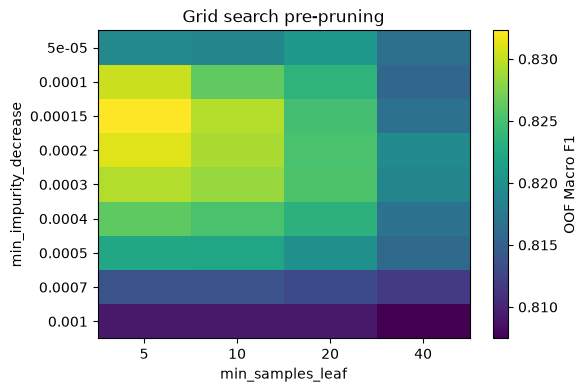
\includegraphics[width=0.48\textwidth]{dtl_grid_gini.png}\hfill
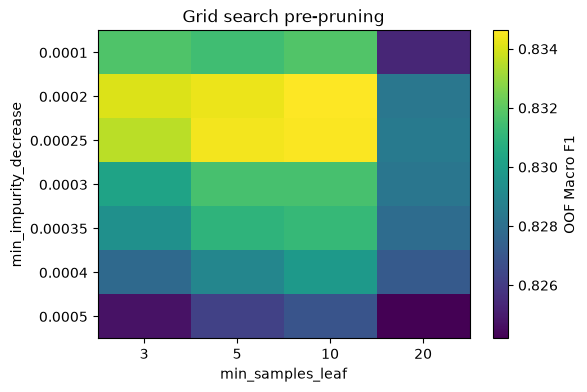
\includegraphics[width=0.48\textwidth]{dtl_grid_gain_ratio.png}
\caption{Grid search pre-pruning (Macro F1 OOF): gini (kiri) dan gain ratio (kanan)}
\label{fig:dtl_grid}
\end{figure}

\begin{table}[H]
\centering
\caption{Decision Tree: from scratch vs scikit-learn pada holdout}
\label{tab:dtl_sklearn}
\begin{tabular}{lrr}
\toprule
Model & Jumlah leaf & Macro F1 holdout \\
\midrule
DTL from scratch (gain ratio) & 273 & \textbf{0,8372} \\
scikit-learn, parameter sama (entropy) & 480 & 0,8297 \\
scikit-learn ID3 (entropy, tanpa batas) & 2.513 & 0,8120 \\
scikit-learn C4.5 (entropy + \texttt{ccp\_alpha} $3\times10^{-4}$) & 343 & 0,8366 \\
scikit-learn CART (gini, tanpa batas) & 2.661 & 0,8063 \\
\bottomrule
\end{tabular}
\end{table}

\begin{table}[H]
\centering
\caption{Cost-complexity pruning pada pohon gain ratio (OOF seed 42)}
\label{tab:dtl_ccp}
\begin{tabular}{rrr}
\toprule
\texttt{ccp\_alpha} & Rata-rata leaf & Macro F1 OOF \\
\midrule
0 sampai $2\times10^{-4}$ & 278 & 0,8343 \\
$3\times10^{-4}$ & 218 & \textbf{0,8348} \\
$5\times10^{-4}$ & 145 & 0,8338 \\
$8\times10^{-4}$ & 96 & 0,8267 \\
$1{,}2\times10^{-3}$ & 61 & 0,8140 \\
\bottomrule
\end{tabular}
\end{table}

\begin{figure}[H]
\centering
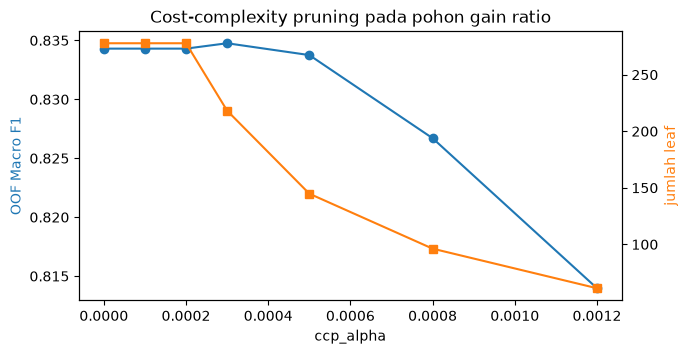
\includegraphics[width=0.65\textwidth]{dtl_ccp.png}
\caption{Cost-complexity pruning: \texttt{ccp\_alpha} terhadap skor dan ukuran pohon}
\label{fig:dtl_ccp}
\end{figure}

\begin{figure}[H]
\centering
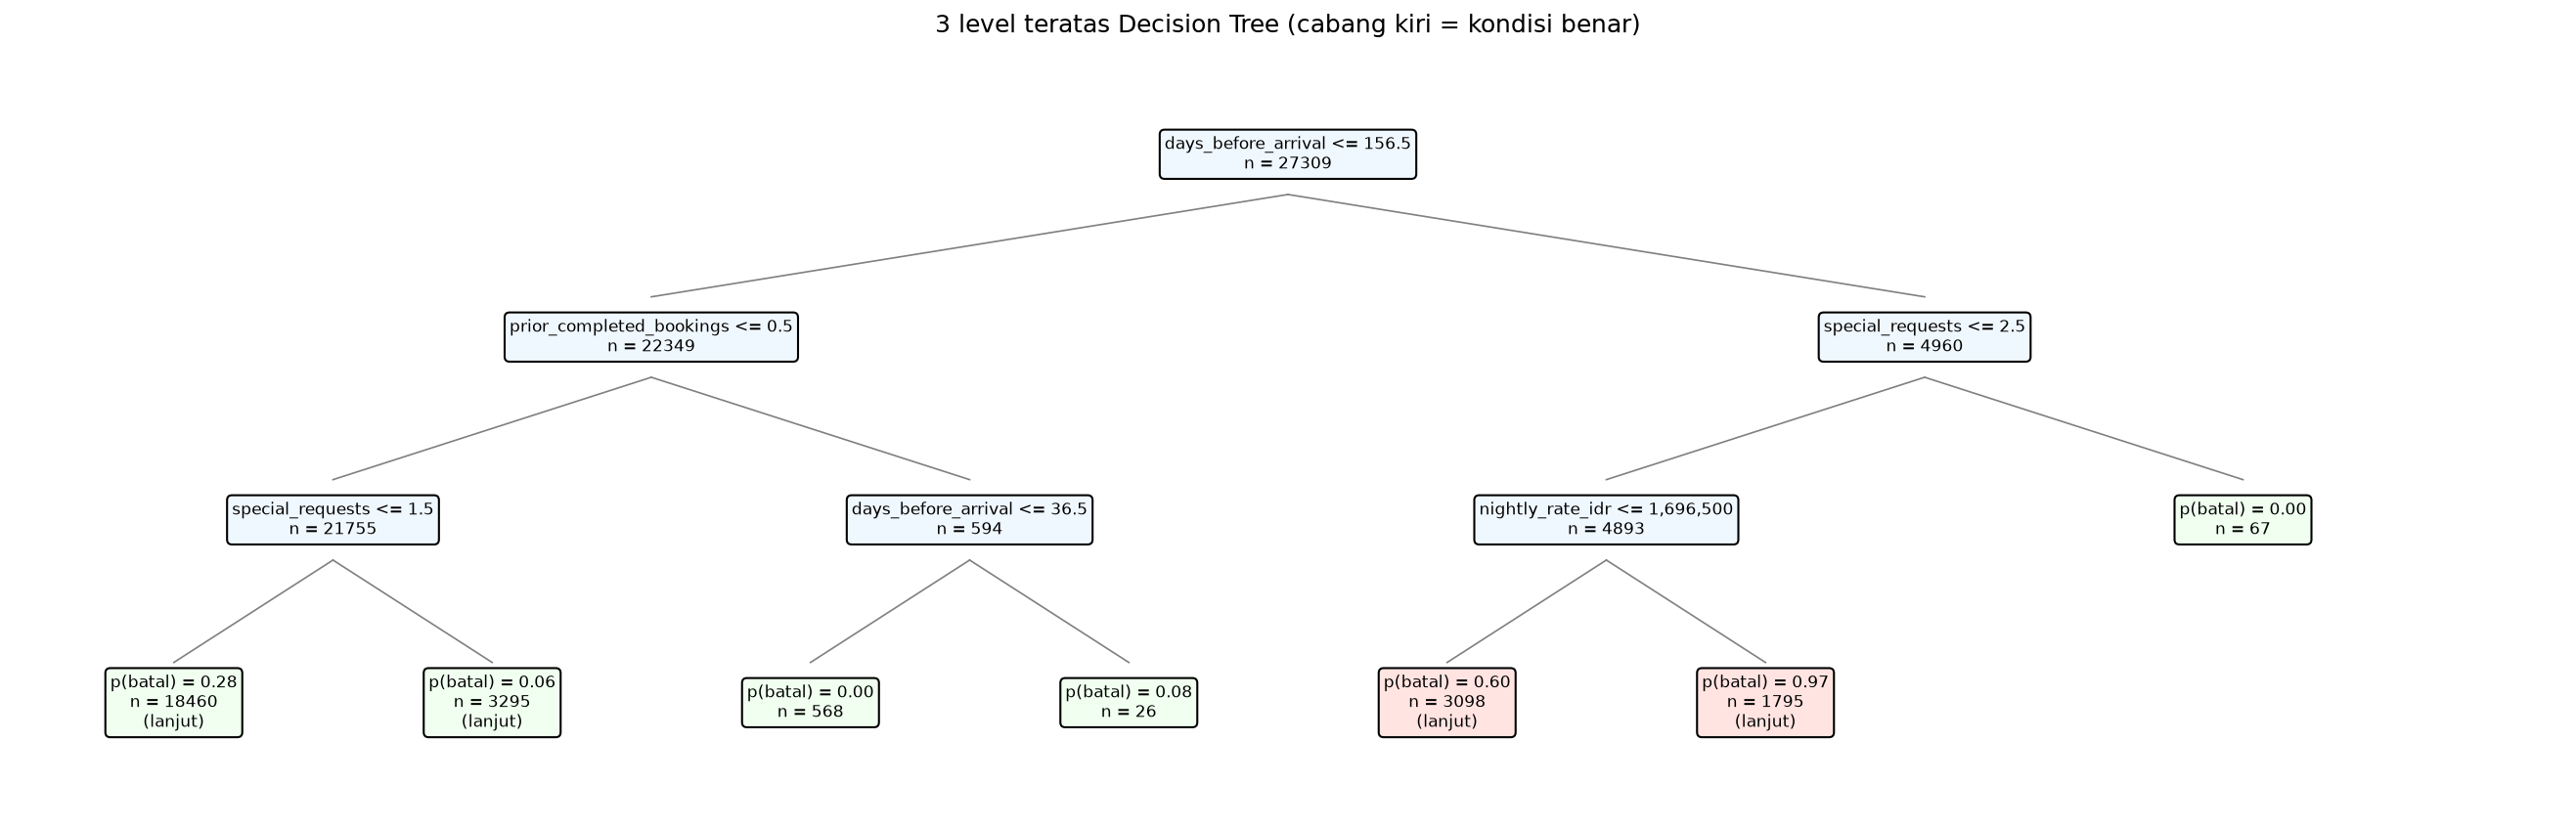
\includegraphics[width=\textwidth]{dtl_tree_top3.png}
\caption{Tiga level teratas pohon DTL final (\texttt{plot\_tree} dengan \texttt{top\_n=3})}
\label{fig:dtl_tree}
\end{figure}

\paragraph{Analisis Decision Tree.}
\begin{enumerate}
  \item \textbf{Pruning paling menentukan.} Pohon tanpa batas (scikit-learn ID3 dan CART, lebih dari 2.500 leaf) paling rendah karena overfit. Pre-pruning dengan minimum gain memangkas pohon dari 459 menjadi 140 leaf sekaligus menaikkan OOF di 5 dari 5 seed fold.
  \item \textbf{Gain ratio paling stabil.} Gain ratio mendapat OOF tertinggi, simpangan baku antar-fold terkecil (0,0028), dan public tertinggi (0,84679). Information gain cenderung memilih split yang memecah data sangat tidak seimbang, sedangkan gain ratio menormalkannya dengan split information.
  \item \textbf{Kenaikan harus dicek di seed lain.} Entropy dengan min gain $4{,}5\times10^{-4}$ naik di seed 42 (0,8332) tetapi turun rata-rata di seed 1 sampai 5 (0,8315 vs 0,8322). Kenaikan di satu pembagian fold dapat hanya kebetulan.
  \item \textbf{Categorical dan missing langsung di pohon.} DTL from scratch membaca 19.933 nilai kosong dan 3 kolom kategorikal tanpa imputasi maupun one-hot, dan unggul atas scikit-learn dengan parameter yang sama yang membutuhkan one-hot dan imputasi (0,8372 vs 0,8297).
  \item \textbf{Cost-complexity pruning.} $\alpha$ sampai $2\times10^{-4}$ tidak memangkas apa pun karena minimum gain $2\times10^{-4}$ sudah mencegah split sekecil itu. $\alpha=3\times10^{-4}$ memangkas 22\% leaf dan sedikit menaikkan OOF, sedangkan $\alpha$ yang terlalu besar menyebabkan underfit. Versi dengan pruning ini mendapat public 0,84604, sedikit di bawah versi tanpa pruning, sehingga model final tetap tanpa pruning.
  \item \textbf{Struktur pohon.} Split pertama adalah lead time 156,5 hari. Pemesanan jauh hari dengan special requests paling banyak 2 dan harga di atas sekitar Rp1,7 juta hampir pasti batal (97\%), sedangkan tamu lama dengan lead time di bawah 37 hari tidak ada yang batal.
\end{enumerate}

\section{Hasil Logistic Regression}

\begin{table}[H]
\centering
\caption{Tahapan tuning Logistic Regression (OOF seed 42)}
\label{tab:lr_tahap}
\begin{tabularx}{\textwidth}{>{\raggedright\arraybackslash}p{3cm}X rr}
\toprule
Tahap & Perubahan & OOF & Public \\
\midrule
baseline & Data tanpa feature engineering, L2 & 0,7595 & -- \\
threshold & + tuning threshold (0,45) & 0,7671 & -- \\
\texttt{lr\_fe} & Bin kuantil, one-hot, interaksi 14 fitur, L2 & 0,8231 & 0,82860 \\
\texttt{lr\_target\_bins} & Bin berbasis target (16 bin), L2 dengan $C=0{,}01$ & 0,8276 & 0,83176 \\
\texttt{lr\_l1\_onehot} & One-hot jumlah tamu, L1 & 0,8297 & 0,83480 \\
\texttt{lr\_cross\_bins} & + sel dua dimensi lead time $\times$ waktu kedatangan, 2.814 kolom & \textbf{0,8344} & \textbf{0,83542} \\
\bottomrule
\end{tabularx}
\end{table}

Dengan preprocessing bersama (28 kolom), Logistic Regression hanya mendapat 0,7644 (\texttt{lr\_main\_prep}). Dengan ekspansi fitur khusus model linear di atas preprocessing bersama (\texttt{lr\_main\_expand}), skornya naik ke 0,8225, dan grid regularisasi menghasilkan L1, L2, dan Elastic Net yang hampir setara (0,8194 sampai 0,8225).

\begin{table}[H]
\centering
\caption{Logistic Regression: from scratch vs scikit-learn (\texttt{lr\_cross\_bins}, holdout)}
\label{tab:lr_sklearn}
\begin{tabular}{lrrrr}
\toprule
Model & Iterasi & Bobot tidak nol & Log-loss & Macro F1 \\
\midrule
From scratch L2 (FISTA) & 1.337 & 2.814 & 0,36342 & 0,8273 \\
From scratch L1 (FISTA) & 432 & 1.234 & 0,33452 & 0,8330 \\
scikit-learn L2 (lbfgs) & 532 & 2.814 & 0,36329 & 0,8272 \\
\bottomrule
\end{tabular}
\end{table}

\begin{figure}[H]
\centering
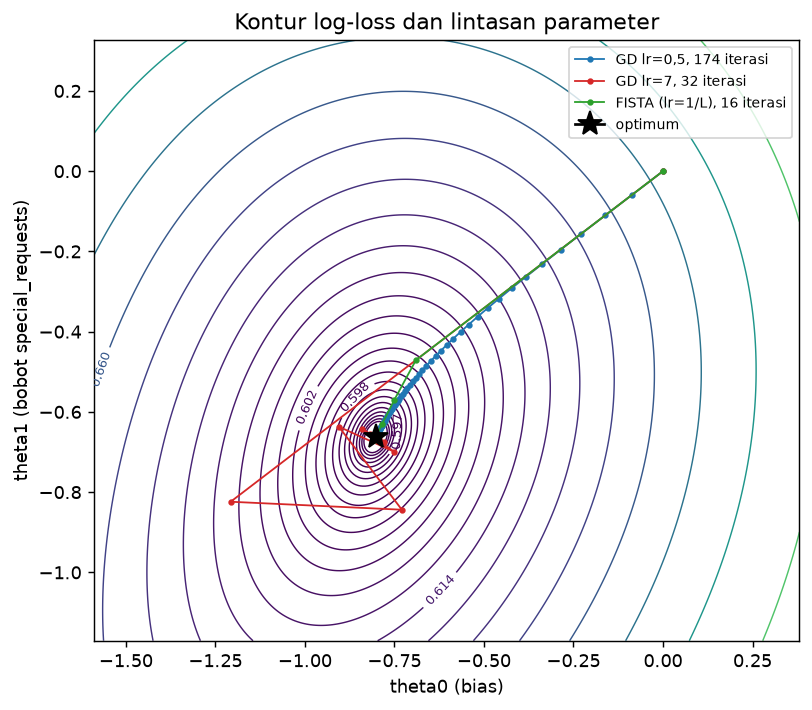
\includegraphics[width=0.75\textwidth]{lr_cross_bins_contour.png}
\caption{Kontur log-loss dan lintasan parameter $(\theta_0,\theta_1)$ selama training (cuplikan video bonus)}
\label{fig:lr_contour}
\end{figure}

\paragraph{Analisis Logistic Regression.}
\begin{enumerate}
  \item \textbf{Kebenaran implementasi.} Objektif L2 from scratch (0,258208) hampir sama dengan scikit-learn (0,258200), dengan Macro F1 holdout 0,8273 vs 0,8272.
  \item \textbf{Model linear butuh representasi tidak linear.} Hubungan lead time dengan pembatalan tidak linear, sehingga satu bobot per fitur tidak cukup. Binning, interaksi, dan sel dua dimensi menaikkan OOF dari 0,7671 ke 0,8344.
  \item \textbf{L1 sebagai seleksi fitur.} Pada 2.814 kolom, L1 hanya mempertahankan 1.234 bobot tidak nol dan memberi log-loss lebih rendah.
  \item \textbf{FISTA lebih cepat.} Pada contoh dua parameter, gradient descent butuh 174 iterasi (learning rate 0,5) atau 32 iterasi (learning rate 7), sedangkan FISTA hanya 16 iterasi untuk mencapai loss yang sama (0,59674).
\end{enumerate}

\section{Hasil Support Vector Machine}
\begingroup
\setlength{\emergencystretch}{3em}
\subsection{Perkembangan eksperimen dan submission}
Eksperimen SVM dimulai dari kernel linear, dilanjutkan dengan tuning linear, Gaussian, polynomial, lalu pipeline final (Tabel~\ref{tab:svm_history}). Empat hasil awal dicatat dengan solver SMO dan seed fold 42. Notebook saat ini sudah memakai dekomposisi SLSQP, tetapi keempat eksperimen tersebut belum seluruhnya dijalankan ulang. SVM final diuji dengan seed 5 dan preprocessing template. Perbedaan ini perlu diperhatikan saat membandingkan kenaikan skor karena pengaruh tiap perubahan belum diuji secara terpisah.
\begin{table}[H]
\centering
\caption{Perkembangan SVM (tanda -- berarti skor public belum teridentifikasi)}
\label{tab:svm_history}
\begin{tabular}{lrrrr}
\toprule
Eksperimen & Threshold & Macro F1 OOF & Std fold & Public \\
\midrule
Linear baseline, $C=0{,}01$ & 0,45 & 0,7656 & 0,0050 & 0,77484 \\
Linear tuning, $C=0{,}1$ & 0,44 & 0,7659 & 0,0053 & -- \\
Gaussian historis, $C=1$ & 0,43 & 0,7907 & 0,0036 & -- \\
Polynomial, $C=1$, $d=3$ & 0,40 & 0,7943 & 0,0034 & 0,81212 \\
\textbf{SVM final}, Gaussian & 0,25 & \textbf{0,83243} & 0,00526 & \textbf{0,85189} \\
\bottomrule
\end{tabular}
\end{table}
Pada eksperimen awal, Gaussian dan polynomial mengungguli linear sekitar 0,025 sampai 0,029 Macro F1. Batas keputusan nonlinear memberi hasil lebih baik pada representasi fitur tersebut. SVM final kemudian naik 0,03809 OOF dan 0,03977 public dibandingkan polynomial awal. Kenaikan ini terjadi setelah preprocessing, konfigurasi, dan seed diubah, sehingga kontribusi masing-masing perubahan masih perlu diperiksa melalui ablation.

Submission SVM final adalah \texttt{output/submissions/submission\_svm\_final.csv}, diterima Kaggle dengan ID \texttt{58803590}, status \texttt{COMPLETE}, dan public score \textbf{0,85189}. Skor private belum tersedia.
Skor public berasal dari sebagian data test di Kaggle, sedangkan OOF dihitung dari train. Selisih keduanya tidak dapat dibandingkan langsung karena datanya berbeda. SVM menjadi submission eksperimen, sementara model final kelompok tetap KNN.

\subsection{Perbandingan dengan scikit-learn dan analisis kesalahan}
\begin{table}[H]
\centering
\caption{Perbandingan penuh SVM final, $C=0{,}3$, $\gamma=1$}
\label{tab:svm}
\begin{tabular}{lrrr}
\toprule
Model & Threshold & Macro F1 OOF & Std fold \\
\midrule
From scratch & 0,25 & 0,832426 & 0,005263 \\
scikit-learn SVC terkalibrasi & 0,27 & 0,832468 & 0,004459 \\
\bottomrule
\end{tabular}
\end{table}
Macro F1 kedua model hanya berselisih 0,000042 pada data, preprocessing, dan fold luar yang sama. Threshold terpilih berbeda karena solver dan cara kalibrasinya dapat menghasilkan probabilitas berbeda. Skor lima fold from scratch berturut-turut adalah 0,82747, 0,82894, 0,83542, 0,82889, dan 0,84139. Semua model fold memenuhi pemeriksaan konvergensi tanpa peringatan. Nilai std dihitung sebagai standar deviasi populasi dari lima skor tersebut dan tidak menyatakan interval kepercayaan.

\begin{figure}[H]
\centering
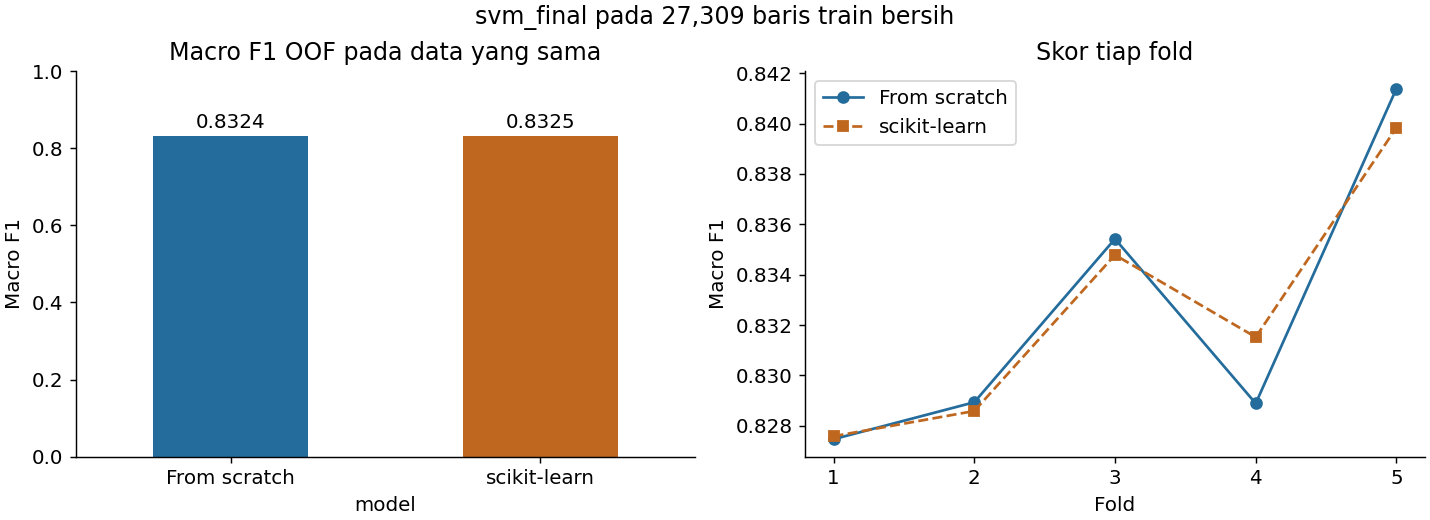
\includegraphics[width=0.78\textwidth]{svm_final_comparison.png}
\caption{Macro F1 OOF dan skor tiap fold SVM final dibandingkan scikit-learn}
\label{fig:svm_comparison}
\end{figure}

Confusion matrix OOF from scratch adalah $\bigl[\begin{smallmatrix}16186&2179\\1886&7058\end{smallmatrix}\bigr]$, dengan urutan baris kelas aktual 0 dan 1 serta kolom kelas prediksi 0 dan 1. Terdapat 2.179 FP dan 1.886 FN. Threshold 0,25 dipilih berdasarkan Macro F1 dari probabilitas yang sudah dikalibrasi. Pemilihan ini belum mempertimbangkan biaya $2FP+FN$. Jumlah FP saja juga belum cukup untuk menilai apakah probabilitas terlalu ekstrem atau kalibrasinya buruk. Eksperimen cost-sensitive kelompok dibahas pada bagian tersendiri dengan model yang digunakan di sana.

\begin{figure}[H]
\centering
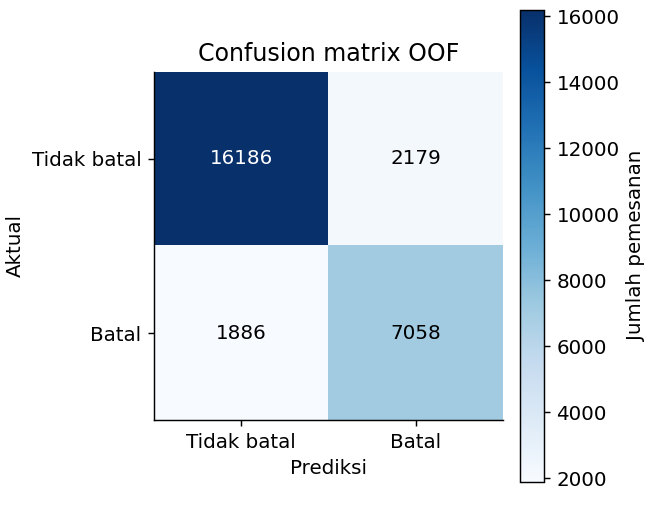
\includegraphics[width=0.61\textwidth]{svm_final_confusion_matrix.png}
\caption{Confusion matrix OOF SVM final dengan threshold 0,25}
\label{fig:svm_confusion}
\end{figure}

\subsection{Bonus bidang pemisah, margin, dan support vector}
Visualisasi ketiga kernel pada Gambar~\ref{fig:svm_boundaries} memakai dua fitur: \texttt{days\_before\_arrival} dan \texttt{nightly\_rate\_idr}. Sebanyak 400 sampel dipilih dengan seed 5, diimputasi median dan distandardisasi berdasarkan sampel visualisasi tersebut. Tiga model dua dimensi dilatih khusus untuk gambar dengan $C=1$, $d=3$, $r=1$, dan \texttt{gamma='scale'} untuk kernel nonlinear. Ketiga model ini dilatih khusus pada dua fitur tersebut. Model submission tetap memakai 28 kolom, dengan konfigurasi dan jumlah support vector yang berbeda.

Garis penuh menunjukkan $f(x)=0$, garis putus-putus menunjukkan $f(x)=\pm1$, dan lingkaran menandai support vector. Warna serta bentuk marker membedakan kelas. Jumlah support vector adalah 226 untuk linear, 207 untuk polynomial, dan 216 untuk Gaussian. Kurva nonlinear mengikuti bentuk yang tidak dapat ditangkap satu garis lurus. Pada soft margin, support vector dapat berada di batas maupun di dalam margin. Untuk kernel nonlinear, jarak antarkontur pada bidang masukan tidak menunjukkan lebar margin Euclidean yang konstan.

\begin{figure}[H]
\centering
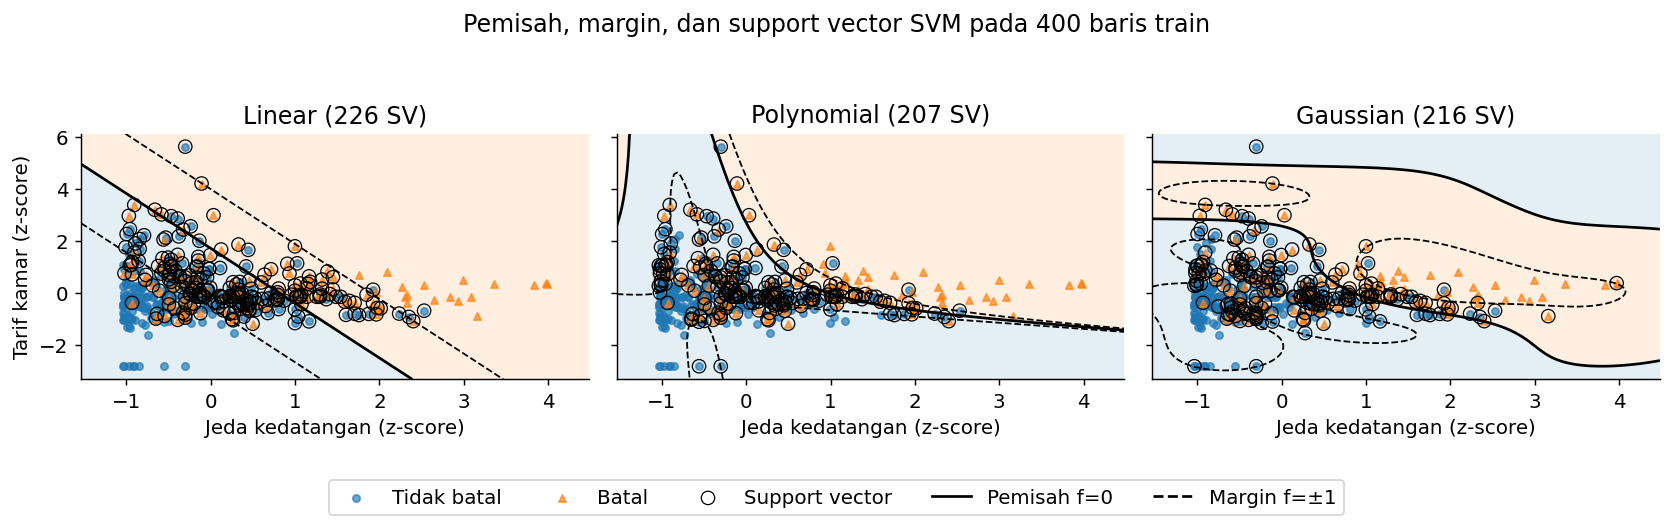
\includegraphics[width=\textwidth]{svm_final_boundaries.png}
\caption{Bidang pemisah, margin, dan support vector pada tiga kernel SVM}
\label{fig:svm_boundaries}
\end{figure}

\subsection{Hasil bonus PSO dan keterbatasan}
\begin{table}[H]
\centering
\caption{PSO pada 800 baris development dan 400 baris holdout}
\label{tab:svm_pso}
\begin{tabular}{lrrrrr}
\toprule
Model & $C$ & $\gamma$ & Threshold & OOF dev & Holdout \\
\midrule
Baseline & 0,30000 & 1,00000 & 0,36 & 0,77046 & 0,80387 \\
PSO terpilih & 0,44287 & 0,49811 & 0,35 & 0,77959 & 0,79404 \\
\bottomrule
\end{tabular}
\end{table}
PSO menyelesaikan 32 evaluasi dalam sekitar 133,7 detik. Skor OOF development naik 0,00913, tetapi skor holdout turun 0,00983. Parameter yang terpilih lebih cocok untuk development dan belum memberi perbaikan pada holdout. Pencarian pada sampel kecil ini masih rentan terhadap bias seleksi. Holdout juga hanya terpisah dalam eksperimen bonus karena pemilihan kernel sebelumnya sudah memakai seluruh train. Dengan satu seed dan ruang pencarian terbatas, hasil PSO belum menjamin konfigurasi terbaik atau peningkatan generalisasi. Karena itu, submission final tetap memakai konfigurasi sebelum PSO.

\begin{figure}[H]
\centering
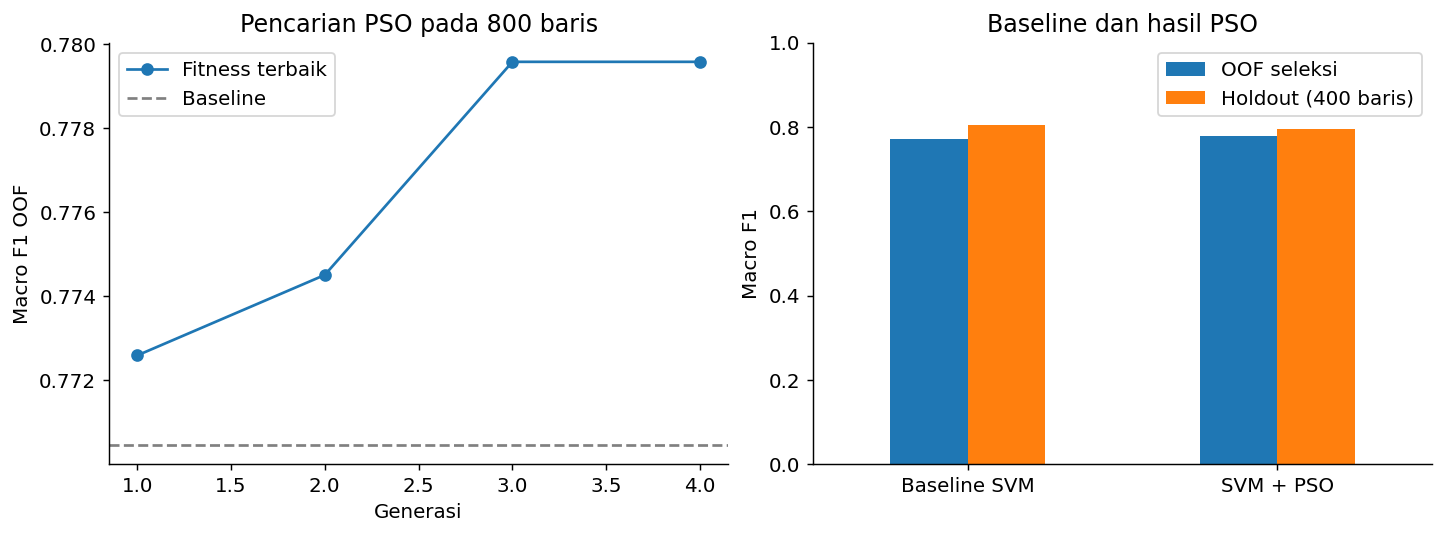
\includegraphics[width=0.95\textwidth]{svm_final_pso.png}
\caption{Perkembangan fitness terbaik PSO serta perbandingan development dan holdout}
\label{fig:svm_pso}
\end{figure}


\endgroup
\section{Hasil Naive Bayes}
\subsection{Perkembangan empat eksperimen}
Tabel~\ref{tab:nb_tahap} membandingkan keempat eksperimen dengan Macro F1 OOF pada protokol tim. Kolom Public memuat skor leaderboard Kaggle untuk baseline 17 fitur, fine-tuning, dan varian kontekstual. Varian dua fitur yang mendahuluinya memakai \texttt{booking\_channel} dan \texttt{special\_requests} dan memperoleh 0,6652 OOF.

\begin{table}[H]
\centering
\caption{Hasil empat eksperimen Naive Bayes pada validasi dan Kaggle}
\label{tab:nb_tahap}
\begin{tabularx}{\textwidth}{p{3.0cm}Xrrrr}
\toprule
Tahap & Perubahan & Threshold & Macro F1 & Std fold & Public \\
\midrule
Baseline & 17 fitur asli, \(\alpha=1\) & 0,42 & 0,73422 & 0,00841 & 0,73697 \\
Fine-tuning & \(\alpha=2\), bobot fitur 2 & 0,49 & 0,73984 & 0,00482 & 0,74192 \\
Smoothing per\newline fitur & \(\alpha=10\) untuk permintaan & 0,49 & 0,73977 & 0,00460 & -- \\
Kontekstual & Bin kontekstual, 9 masukan & 0,43 & \textbf{0,80196} & 0,00729 & \textbf{0,80173} \\
\bottomrule
\end{tabularx}
\end{table}

\begin{figure}[htbp]
\centering
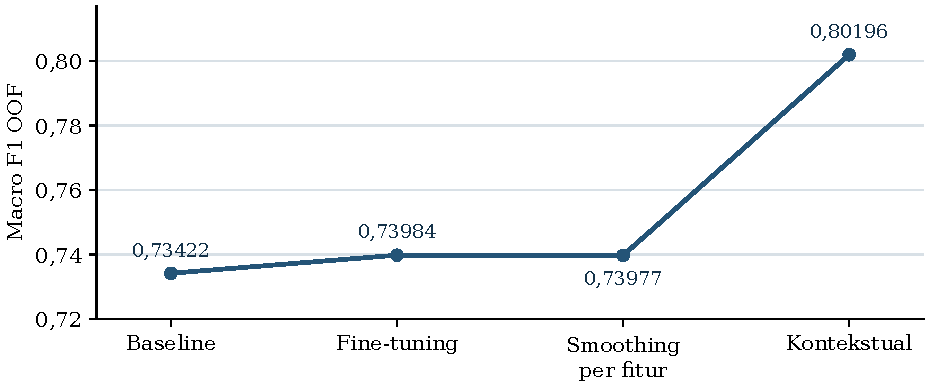
\includegraphics[width=0.84\textwidth]{nb_macro_f1.pdf}
\caption{Perubahan Macro F1 OOF antar-eksperimen pada protokol tim.}
\label{fig:nb_oof}
\end{figure}

Fine-tuning menaikkan Macro F1 sebesar 0,00562 dan memperbaiki empat dari lima fold. Dibanding baseline, false positive turun dari 3.917 ke 3.252, sedangkan false negative naik dari 2.688 ke 3.044. Smoothing per fitur menghasilkan perubahan total \(-0{,}00007\), walaupun tiga fold membaik tipis. Pada konfigurasi ini, smoothing yang lebih kuat untuk satu fitur belum menambah daya prediksi. Perubahan terbesar muncul pada tahap kontekstual, dengan kenaikan 0,06219 terhadap tahap sebelumnya. Karena tahap tersebut sekaligus mengubah diskretisasi, susunan fitur, dan pemilihan parameter, selisihnya mengukur efek gabungan.

\subsection{Validasi bertingkat dan perbandingan dengan scikit-learn}
Konfigurasi ekspor memperoleh OOF seleksi 0,80328 dengan threshold 0,45. Skor ini ikut menentukan konfigurasi yang dipilih. Validasi bertingkat memperoleh 0,79943 pada gabungan prediksi fold luar dan unggul pada lima fold terhadap \texttt{nb\_categorical\_tuned}, pembanding lama yang memakai bin hari rinci, kuantil tarif, dan gabungan kanal dengan rentang hari. Pembanding tersebut menggunakan prosedur validasi bertingkat yang sama dan berbeda dari baseline 17 fitur pada Tabel~\ref{tab:nb_tahap}.

\begin{table}[H]
\centering
\caption{Macro F1 pada fold luar validasi bertingkat kontekstual}
\label{tab:nb_nested}
\begin{tabular}{lrrr}
\toprule
Fold luar & Pembanding lama & Kontekstual & Threshold kontekstual \\
\midrule
1 & 0,75828 & 0,81082 & 0,435 \\
2 & 0,75328 & 0,79016 & 0,450 \\
3 & 0,75488 & 0,79297 & 0,475 \\
4 & 0,75433 & 0,80747 & 0,460 \\
5 & 0,74997 & 0,79571 & 0,420 \\
\midrule
OOF gabungan & 0,75421 & \textbf{0,79943} & -- \\
\bottomrule
\end{tabular}
\end{table}

\begin{table}[H]
\centering
\caption{Kesetaraan from scratch dengan pembanding scikit-learn pada konfigurasi yang sama}
\label{tab:nb}
\begin{tabularx}{\textwidth}{Xrrr}
\toprule
Tahap & From scratch & Pembanding & Selisih peluang maks. \\
\midrule
Baseline & 0,73422 & 0,73422 & \(6{,}00\times 10^{-15}\) \\
Fine-tuning (likelihood berbobot) & 0,73984 & 0,73984 & \(5{,}33\times 10^{-15}\) \\
Smoothing per fitur (likelihood berbobot) & 0,73977 & 0,73977 & \(5{,}44\times 10^{-15}\) \\
Kontekstual (OOF seleksi) & 0,80328 & 0,80328 & \(4{,}66\times 10^{-15}\) \\
\bottomrule
\end{tabularx}
\end{table}

Pada fine-tuning, \texttt{CategoricalNB} standar dengan bobot seragam dan \(\alpha=2\) memperoleh 0,73380. Pembanding berbobot memperoleh 0,73984. Selisih peluang pada Tabel~\ref{tab:nb} setara dengan galat pembulatan. Baris kontekstual memakai OOF seleksi karena verifikasi memakai konfigurasi ekspor dan fold yang sama.

\subsection{Analisis kesalahan, reproduksibilitas, dan bonus}
Prediksi gabungan fold luar kontekstual menghasilkan 15.960 \emph{true negative}, 2.444 \emph{false positive}, 2.400 \emph{false negative}, dan 6.569 \emph{true positive}. F1 kelas tidak batal mencapai 0,86824, sedangkan F1 kelas batal mencapai 0,73062. Pada kelompok \emph{lead time} lebih dari 80 hingga 151 hari, tingkat kesalahan masih 25,7\% dari 5.191 baris. Kelompok 11 hari atau kurang memiliki tingkat kesalahan 9,9\% dari 5.293 baris. Hasil ini menunjukkan bahwa kualitas prediksi berbeda antar-kelompok pemesanan setelah diskretisasi kontekstual.

Hasil run ulang \texttt{nb\_baseline} identik byte demi byte dengan \texttt{submission\_nb\_categorical\_all.csv} di branch \texttt{main}, yang mencatat public score 0,73697. Fine-tuning mencapai 0,74192 pada public leaderboard. Varian kontekstual mencapai 0,80173 dengan 6.844 prediksi dan threshold ekspor 0,45. Skor kontekstual 0,80196 dan 0,79943 berasal dari validasi data latih. KNN dengan vote booking kembar tetap menjadi model submission final kelompok.

Gambar~\ref{fig:nb_graf} menampilkan struktur dari sel bonus notebook kontekstual dengan label ringkas. Simpul \texttt{is\_canceled} memiliki sembilan anak sesuai masukan model. Panah menjelaskan faktorisasi peluang kondisional. Masing-masing simpul dapat berupa satu fitur atau satu kategori gabungan.

\begin{figure}[H]
\centering
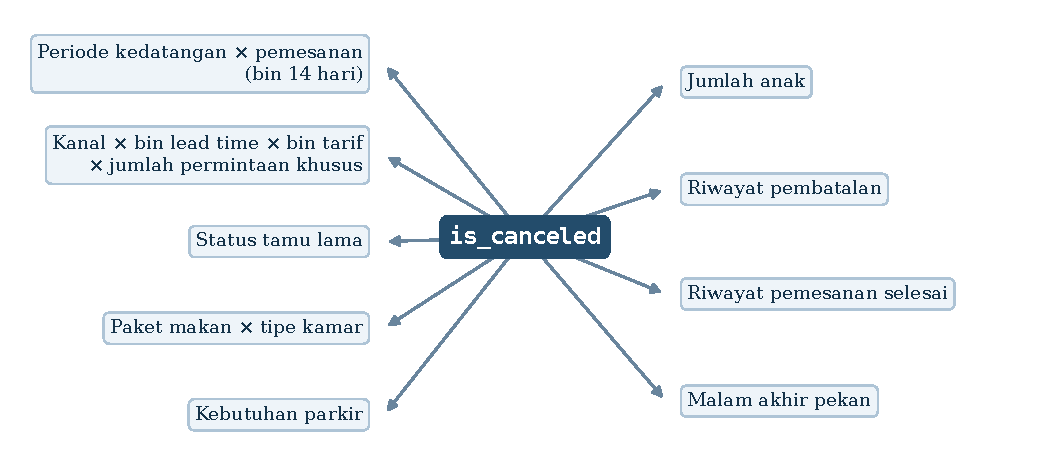
\includegraphics[width=\textwidth]{nb_graf.pdf}
\caption{Graf Bayesian Network untuk konfigurasi Categorical Naive Bayes kontekstual.}
\label{fig:nb_graf}
\end{figure}


\section{Analisis Perbandingan Antar-Model}
\begin{enumerate}
  \item \textbf{Peringkat.} KNN + kembar (0,8529) $>$ KNN (0,8476) $>$ DTL ($\approx$0,834) $\approx$ LR ($\approx$0,834) $>$ SVM final (0,8324) $>$ NB kontekstual (0,8020). Skor public SVM final (0,85189) melebihi DTL dan LR pada tabel ringkasan, sehingga urutan public tidak seluruhnya sama dengan urutan OOF. Skor public NB kontekstual adalah 0,80173. Perbedaan seed dan prosedur seleksi membatasi perbandingan langsung.
  \item \textbf{Representasi fitur lebih menentukan daripada algoritma.} KNN naik dari 0,7632 ke 0,8476 dan LR dari 0,7595 ke 0,8344 hanya dengan mengubah representasi fitur. Decision Tree kuat tanpa banyak rekayasa fitur karena seleksi fitur sudah melekat pada pemilihan split.
  \item \textbf{Memahami cara data dibuat.} Kenaikan terbesar KNN final datang dari analisis noise: pemesanan kembar hampir selalu berlabel sama, dan noise ada pada lead time. Informasi ini dipakai langsung lewat vote kembar.
  \item \textbf{Threshold menggantikan resampling.} Threshold OOF SVM final adalah 0,25, sedangkan banyak eksperimen lain berada sekitar 0,40 sampai 0,53. Karena kelas batal hanya 32,8\%, menurunkan threshold menyeimbangkan recall kelas minoritas dan menaikkan Macro F1 tanpa data sintetis.
  \item \textbf{Kesetaraan dengan pustaka.} Implementasi from scratch setara dengan scikit-learn: KNN dan Naive Bayes identik secara numerik, LR berselisih 0,0001, dan DTL dengan cost-complexity pruning menghasilkan pohon yang sama persis dengan scikit-learn pada parameter yang sama.
\end{enumerate}

\section{Cost-sensitive Classification}
False Positive (diprediksi batal, ternyata datang) lebih mahal karena penginapan dapat overbooked. Diasumsikan biaya FP dua kali FN, sehingga total biaya adalah $2\,FP + FN$. Dengan probabilitas yang terkalibrasi, keputusan dengan biaya harapan minimum adalah memprediksi batal jika $\hat{p}\,C_{FN} > (1-\hat{p})\,C_{FP}$, yaitu $\hat{p} > C_{FP}/(C_{FP}+C_{FN}) = 2/3$ \cite{ref:elkan}. Threshold juga dicari langsung dari prediksi OOF model final.

\begin{table}[H]
\centering
\caption{Pengaruh threshold pada biaya (OOF KNN + kembar)}
\label{tab:cost}
\begin{tabular}{lrrrrrr}
\toprule
Threshold & Nilai & FP & FN & Biaya & Macro F1 & Prediksi batal \\
\midrule
Macro F1 maksimum & 0,4845 & 1.637 & 1.877 & 5.151 & 0,8529 & 31,9\% \\
Teori $2/3$ & 0,6667 & 764 & 2.931 & 4.459 & 0,8350 & 24,8\% \\
Biaya minimum (OOF) & 0,74 & 494 & 3.423 & \textbf{4.411} & 0,8197 & 22,0\% \\
\bottomrule
\end{tabular}
\end{table}

\begin{figure}[H]
\centering
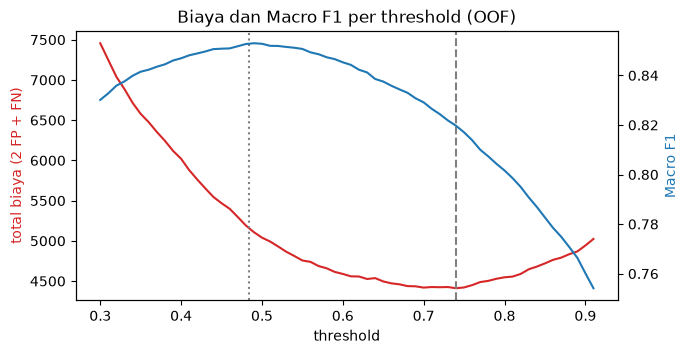
\includegraphics[width=0.65\textwidth]{cost_sensitive.png}
\caption{Total biaya dan Macro F1 terhadap threshold}
\label{fig:cost}
\end{figure}

Dengan biaya FP dua kali FN, threshold dinaikkan dari 0,4845 ke sekitar 0,67 sampai 0,74, dan biaya turun 14\%. FP turun dari 1.637 ke 494, tetapi FN naik dari 1.877 ke 3.423 dan Macro F1 turun ke 0,8197. Model dan preprocessing tidak berubah, yang berubah hanya threshold keputusan. Threshold empiris (0,74) dekat dengan teori (0,67), menandakan probabilitas model cukup terkalibrasi. Untuk kompetisi tetap dipakai threshold Macro F1 karena metrik Kaggle adalah Macro F1.

\section{Ringkasan Bonus}
\begin{table}[H]
\centering
\caption{Bonus yang dikerjakan}
\label{tab:bonus}
\begin{tabularx}{\textwidth}{>{\raggedright\arraybackslash}p{4.2cm}X}
\toprule
Bonus & Keterangan \\
\midrule
Kaggle & Peringkat 1 public leaderboard dengan KNN from scratch, reproducible melalui \texttt{src/main.ipynb} \\
DTL: gambar percabangan & \texttt{plot\_tree(model, top\_n)}, Gambar~\ref{fig:dtl_tree}, berkas \texttt{output/figures/dtl\_tree\_top3.png} \\
LR: video kontur log-loss & \texttt{output/figures/lr\_*\_contour.mp4}, Gambar~\ref{fig:lr_contour} \\
SVM: gambar bidang pemisah & Linear, polynomial, dan Gaussian, termasuk margin serta support vector pada Gambar~\ref{fig:svm_boundaries}, dengan kode pada \texttt{svm\_final.ipynb} \\
Naive Bayes: graf fitur & Graf untuk sembilan masukan kategori terpilih, Gambar~\ref{fig:nb_graf} \\
Algoritma optimasi DTL & Cost-complexity pruning \cite{ref:breiman}, Tabel~\ref{tab:dtl_ccp} \\
Algoritma optimasi LR & FISTA dengan adaptive restart \cite{ref:fista}, Kode~\ref{lst:fista} \\
Algoritma optimasi SVM & PSO untuk $C$ dan $\gamma$, Kode~\ref{lst:svm_pso}, dan Tabel~\ref{tab:svm_pso}. Fitness naik tetapi holdout turun \cite{ref:pso,ref:pso_shi} \\
Algoritma optimasi NB & Diskretisasi MDL, penggabungan kategori, dan seleksi wrapper \cite{ref:fayyad_nb,ref:pazzani_nb,ref:kohavi_nb}, Tabel~\ref{tab:nb_nested} \\
Cost-sensitive classification & Tabel~\ref{tab:cost} \\
\bottomrule
\end{tabularx}
\end{table}
